\documentclass{standalone}

\usepackage{standalone}
\usepackage{tikz}
\usetikzlibrary{calc,intersections}

\begin{document}
	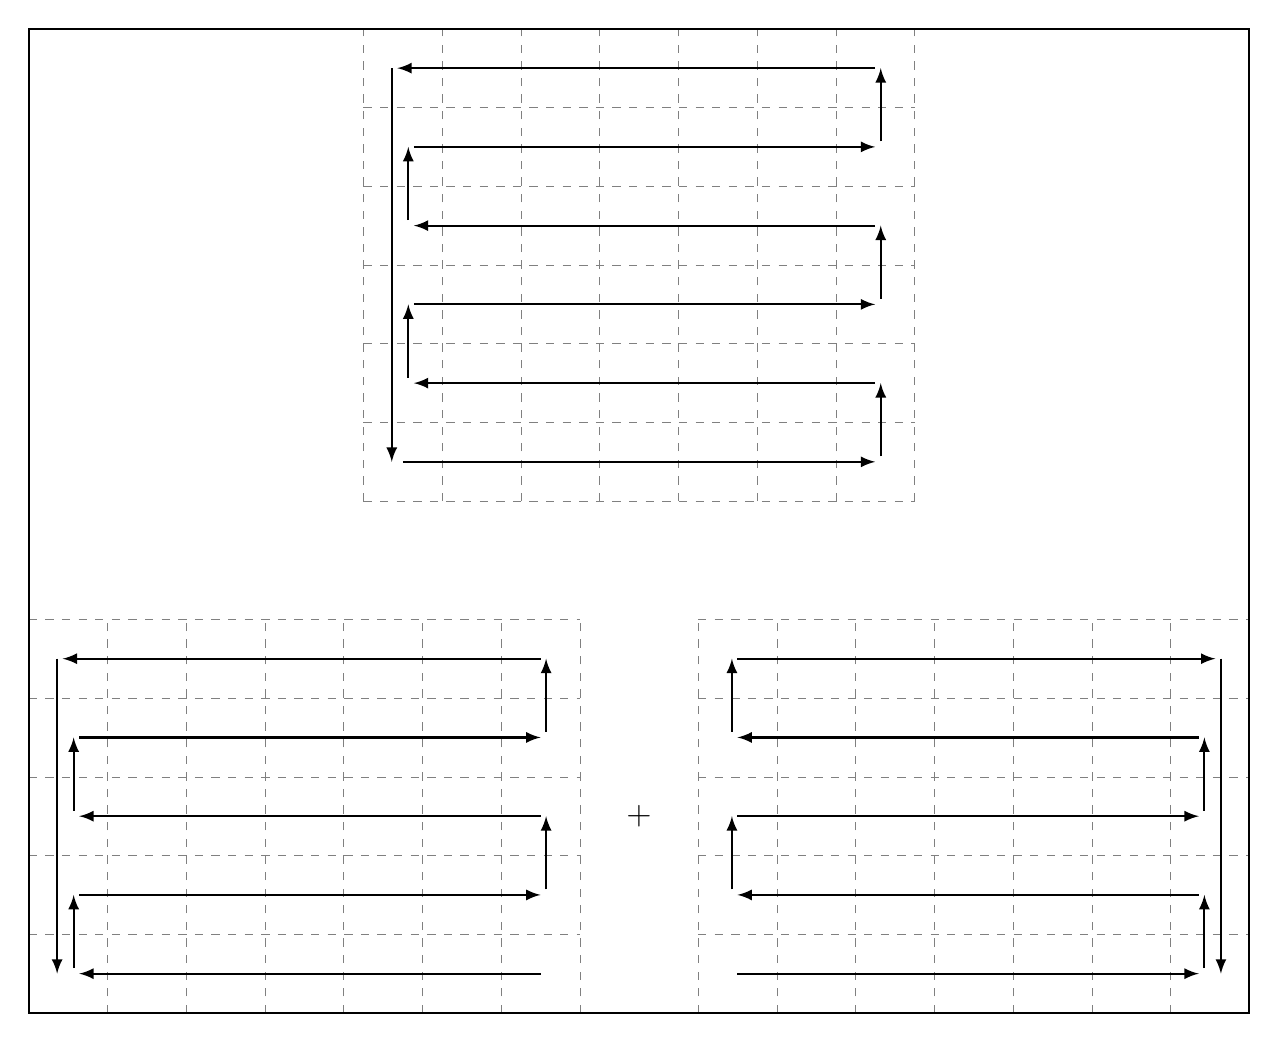
\begin{tikzpicture}
	
		\pgfmathtruncatemacro{\xsize}{7}
		\pgfmathtruncatemacro{\ysize}{6}


		\pgfmathsetmacro{\arrowoffset}{0.07}
		\pgfmathsetmacro{\intergriddistance}{1.5}
		
		% draw even n grid
		\draw[dashed, very thin, black!50] (0,0) grid (\xsize, \ysize);

		% draw odd n grid
		\begin{scope}[shift={(-\xsize / 2 - \intergriddistance / 2 , -\ysize - \intergriddistance + 1)}]
			% draw left grid
			\draw[dashed, very thin, black!50] (0,0) grid (\xsize, \ysize - 1);
			% draw right grid
			\begin{scope}[shift = {({\xsize + \intergriddistance}, 0)}]
				\draw[dashed, very thin, black!50] (0,0) grid (\xsize, \ysize - 1);
			\end{scope}
			\node at (\xsize + \intergriddistance / 2, \ysize / 2 - 1 / 2) {\large +};
		\end{scope}
		
		\draw[thick] 
			(-\xsize / 2 - \intergriddistance / 2, \ysize) --
			++(2 * \xsize + \intergriddistance, 0) --
			++(0, - 2 * \ysize -  \intergriddistance + 1) --
			++(-2 * \xsize - \intergriddistance, 0) --
			cycle;

		\pgfmathtruncatemacro{\xinnersize}{\xsize - 2}
		\pgfmathtruncatemacro{\yinnersize}{\ysize - 2}
		
		% draw even path
		\begin{scope}[shift={(0.5, -0.5)}, thick]
			\foreach \row in {1, ..., \ysize}
			{
				\pgfmathtruncatemacro{\direction}{Mod(\row, 2)}
				\ifnum\direction=1 % right
					\ifnum\row=1
						\draw[-latex] (0, \row) -- ++(\xinnersize + 1, 0); % arrow right
					\else
						\draw[-latex] (0 + 2 * \arrowoffset, \row) -- ++(\xinnersize + 1 - 2 * \arrowoffset, 0); % arrow right
					\fi
					\draw[-latex] (\xinnersize + 1 + \arrowoffset, \row + \arrowoffset) -- ++(0, 1 - \arrowoffset); % arrow up
				\else % left
					\ifnum\row=\ysize
						\draw[-latex] (\xinnersize + 1, \row) -- (0 - \arrowoffset, \row); % arrow left
					\else
						\draw[-latex] (\xinnersize + 1, \row) -- (0 + 2 * \arrowoffset, \row); % arrow left
					\fi
					\ifnum\row<\ysize
						\draw[-latex] (\arrowoffset, \row + \arrowoffset) -- ++(0, 1 - \arrowoffset); % arrow up
					\fi
				\fi
			}
			\draw[-latex] (0 - 2 * \arrowoffset, \ysize) -- ++(0, -\ysize + 1); % arrow down
		\end{scope}
		
		% draw odd row path
		\begin{scope}[shift={(-\xsize / 2 - \intergriddistance / 2 , -\ysize - \intergriddistance + 1)}]
			% draw in the left grid
			\begin{scope}[shift={(0.5, 0.5)}, thick]
				\foreach \row in {0, ..., \yinnersize}
				{
					\pgfmathtruncatemacro{\direction}{Mod(\row, 2)}
					\ifnum\direction=1 % right
						\draw[-latex] (0 + 2 * \arrowoffset, \row) -- ++(\xinnersize + 1 - 2 * \arrowoffset, 0); % arrow right
						\draw[-latex] (\xinnersize + 1 + \arrowoffset, \row + \arrowoffset) -- ++(0, 1 - \arrowoffset); % arrow up
					\else % left
						\ifnum\row=\yinnersize
							\draw[-latex] (\xinnersize + 1, \row) -- (0 - \arrowoffset, \row); % arrow left
						\else
							\draw[-latex] (\xinnersize + 1, \row) -- (0 + 2 * \arrowoffset, \row); % arrow left
						\fi
						\ifnum\row<\yinnersize
							\draw[-latex] (\arrowoffset, \row + \arrowoffset) -- ++(0, 1 - \arrowoffset); % arrow up
						\fi
					\fi
				}
				\draw[-latex] (0 - 2 * \arrowoffset, \yinnersize) -- ++(0, -\yinnersize); % arrow down
			% draw in the right grid			
				\begin{scope}[shift = {({2 * \xsize + \intergriddistance - 1}, 0)}, thick]
					\begin{scope}[yscale=1,xscale=-1]
						\foreach \row in {0, ..., \yinnersize}
						{
							\pgfmathtruncatemacro{\direction}{Mod(\row, 2)}
							\ifnum\direction=1 % right
								\draw[-latex] (0 + 2 * \arrowoffset, \row) -- ++(\xinnersize + 1 - 2 * \arrowoffset, 0); % arrow right
								\draw[-latex] (\xinnersize + 1 + \arrowoffset, \row + \arrowoffset) -- ++(0, 1 - \arrowoffset); % arrow up
							\else % left
								\ifnum\row=\yinnersize
									\draw[-latex] (\xinnersize + 1, \row) -- (0 - \arrowoffset, \row); % arrow left
								\else
									\draw[-latex] (\xinnersize + 1, \row) -- (0 + 2 * \arrowoffset, \row); % arrow left
								\fi
								\ifnum\row<\yinnersize
									\draw[-latex] (\arrowoffset, \row + \arrowoffset) -- ++(0, 1 - \arrowoffset); % arrow up
								\fi
							\fi
						}
						\draw[-latex] (0 - 2 * \arrowoffset, \yinnersize) -- ++(0, -\yinnersize); % arrow down
					\end{scope}
				\end{scope}
			\end{scope}
		\end{scope}
	\end{tikzpicture}
\end{document}
